\newcommand{\ra}[1]{\renewcommand{\arraystretch}{#1}}
\newcommand*{\Scale}[2][4]{\scalebox{#1}{$#2$}}%
\newcommand\scalemath[2]{\scalebox{#1}{\mbox{\ensuremath{\displaystyle #2}}}}

\newcommand{\gev}{\,\textrm{GeV}}
\newcommand{\tr}{{\rm Tr}}
\newcommand{\del}{\partial}
\newcommand{\sgn}{\operatorname{sgn}}
\newcommand{\e}{\mathrm e}
\renewcommand{\d}{\mathrm d}
\renewcommand{\i}{\mathrm i}
\renewcommand{\(}{\left(}
\renewcommand{\)}{\right)}
\renewcommand{\[}{\left[}
\renewcommand{\]}{\right]}
\newcommand{\VSl}[3]{(\langle \tilde{L} \rangle ^{ #1} )^{ #2 }{}_{ #3 }}
\newcommand{\Sl}[3]{(\tilde{L}^{ #1} )^{ #2 }{}_{ #3 }}
\newcommand{\SlS}[3]{(\tilde{L}^*_{ #1} )_{ #2 }{}^{ #3 }}

\newcommand{\U}[1]{\mathrm{U}(1)_{\mathrm{#1}}}			% Use this for U(1) groups
\newcommand{\SU}[2]{\mathrm{SU}(#1)_{\mathrm{#2}}}		% Use this for SU(N) groups
\newcommand{\SO}[2]{\mathrm{SO}(#1)_{\mathrm{#2}}}		% Use this for SO(N) groups
\newcommand{\E}[1]{\mathrm{E}_{#1}}		% Use this for Exeptional groups
\newcommand{\T}[2]{T_{\mathrm{#1}}^{#2}}
\newcommand{\Q}[1]{\hat{Q}_{\mathrm{#1}}}				% Use this for generators	
\newcommand{\RN}[1]{%
	\textup{\uppercase\expandafter{\romannumeral#1}}%
}

% SUPERFIELDS
\newcommand{\LLR}[3]{\left(L^{ #1} \right)^{ #2 }{}_{ #3 }}
\newcommand{\QL}[3]{\left(Q_\mathrm{L}^{ #1} \right)^{ #2 }{}_{ #3 }}
\newcommand{\QR}[3]{\left(Q_\mathrm{R}^{ #1} \right)^{ #2 }{}_{ #3 }}

%FERMIONS
\newcommand{\LLRs}[3]{\left(L^*_{ #1} \right)_{ #2 }{}^{ #3 }}
\newcommand{\QLs}[3]{\left(Q^*_{\mathrm{L} #1} \right)_{ #2 }{}^{ #3 }}
\newcommand{\QRs}[3]{\left(\overline{Q}^*_{\mathrm{R} #1} \right)_{ #2 }{}^{ #3 }}


\newcommand{\FLLR}[3]{\big(L^{ #1} \big)^{ #2 }{}_{ #3 }}
\newcommand{\FQL}[3]{\big(Q_{\mathrm{L}}^{ #1} \big)^{ #2 }{}_{ #3 }}
\newcommand{\FQR}[3]{\big(Q_{\mathrm{R}}^{ #1} \big)^{ #2 }{}_{ #3 }}
\newcommand{\FDA}[2]{\Delta_{\mathrm{#1}}^{ #2}}

\newcommand{\FLLRd}[3]{\big(L^{\dagger}_{ #1} \big)_{ #2 }{}^{ #3 }}
\newcommand{\FQLd}[3]{\big(Q_{\mathrm{L}}^ {\dagger}{}_{ #1} \big)_{ #2 }{}^{ #3 }}
\newcommand{\FQRd}[3]{\big(Q_{\mathrm{R}}^{\dagger}{}_{ #1} \big)_{ #2 }{}^{ #3 }}
\newcommand{\FDAd}[2]{\Delta^{\dagger}_{\mathrm{#1}}{}^{ #2}}

%SCALARS
\newcommand{\SLLR}[3]{\left(\tilde{L}^{ #1} \right)^{ #2 }{}_{ #3 }}
\newcommand{\SQL}[3]{\left(\tilde{Q}_\mathrm{L}^{ #1} \right)^{ #2 }{}_{ #3 }}
\newcommand{\SQR}[3]{\left(\tilde{Q}_\mathrm{R}^{ #1} \right)^{ #2 }{}_{ #3 }}
\newcommand{\SLLRs}[3]{\left(\tilde{L}^*_{ #1} \right)^{ #3 }{}_{ #2 }}
\newcommand{\SQLs}[3]{\left(\tilde{Q}^*_{\mathrm{L} #1} \right)^{ #3 }{}_{ #2 }}
\newcommand{\SQRs}[3]{\left(\tilde{Q}^*_{\mathrm{R} #1} \right)_{ #3 }{}^{ #2 }}

\newcommand{\lam}[2]{\lambda_{\Scale[0.6]{#1 \-- #2}}}
\newcommand{\la}[1]{\lambda_{\Scale[0.6]{#1}}}
\newcommand{\lab}[1]{\bar{\lambda}_{\Scale[0.6]{#1}}}
\newcommand{\y}[1]{\mathrm{y}_{\Scale[0.6]{#1}}}
\newcommand{\mean}[1]{\left \langle #1 \right \rangle }
\newcommand{\vev}[1]{v_{\mathrm{#1}}}
\newcommand{\abs}[1]{\left| #1 \right| }
\newcommand{\g}[2]{g_{_\mathrm{#1}}^{#2}}

\newcommand{\blue}[0]{\color{blue}}
\newcommand{\green}[0]{\color{ForestGreen}}
\newcommand{\red}[0]{\color{red}}
\newcommand{\magenta}[0]{\color{magenta}}
\newcommand{\brown}[0]{\color{brown}}
\newcommand{\cyan}[0]{\color{cyan}}
\newcommand{\purple}[0]{\color{purple}}


\newcommand{\bfrac}[2]{\displaystyle\frac{#1}{#2}}
\newcommand{\conj}[1]{\ensuremath{#1^*}}

\documentclass[10pt,xcolor=dvipsnames,mathserif]{beamer} 

\usetheme{Copenhagen}

\graphicspath{{Images/}}

\useoutertheme{infolines} 

\usepackage{bm} % bold greek simbols
\usepackage{multicol}
\usepackage{slashed}

\setbeamertemplate{headline}[infolines theme] 
%\setbeamertemplate{footline}[page number]
\setbeamertemplate{footline}[infolines theme] 
\setbeamertemplate{items}[ball] 
\setbeamertemplate{blocks}[rounded][shadow=true] 
\setbeamertemplate{navigation symbols}{} 


\setbeamercolor{structure}{fg=blue!25!black} 
%\setbeamercolor{foot1}{fg=white, bg=red!65!black} 
%\setbeamercolor{foot2}{fg=white, bg=blue!25!black} 
%\setbeamercolor{foot3}{fg=white, bg=red!65!black} 

\titlegraphic{
	\vskip-5mm
	
\includegraphics[height=1.5cm,width=2cm,keepaspectratio]{Logos/logoAveiro.jpg}\hspace*{0.8cm}~%
	\vspace{-.5cm}\hspace*{-1cm}
\includegraphics[height=1.5cm,width=2cm,keepaspectratio]{Logos/2017_FCT_H_cor.jpg}\hspace*{-0.3cm}~%
	%\includegraphics[width=8mm]{logoLund.png}\hspace*{0.8cm}~
	
\includegraphics[width=60mm]{Logos/logoProj.jpeg}\hspace*{0.05cm}~
	
\includegraphics[height=1.5cm,width=2cm,keepaspectratio]{Logos/cost.jpg}
	%
	
}

\title{Phenomenological analysis in beyond the Standard Model theories: the cases of the minimal B-L-SM and of a BGL-like 3HDM}

\author{\textbf{Pedro Rodrigues}}

\date{\today}

\institute{Universidade de Aveiro}


\begin{document}
% creating the front slide 
% titles and contents 
% \section{Starting Pages}

\begin{frame}
	\titlepage
	% equivalent to:
	% \maketitle
\end{frame}

\begin{frame}
	\frametitle{General Structure}
	\tableofcontents
\end{frame}	

\section{SM Introduction}

\subsection{Introduction - Context}

\begin{frame}
	\frametitle{The Standard Model - And it's unfortunate problems}
	\begin{itemize}
		\item The Standard Model (\textbf{SM}) is a great \textbf{approximation} \pause ... but what exactly is the \textbf{SM}? 
		\pause
		\item It can be described as a QFT theory that unifies the strong weak and color force.  
	\end{itemize}
	\pause
	However things can be more complicated than that... the full SM Lagrangian is,  
	\begin{figure}
		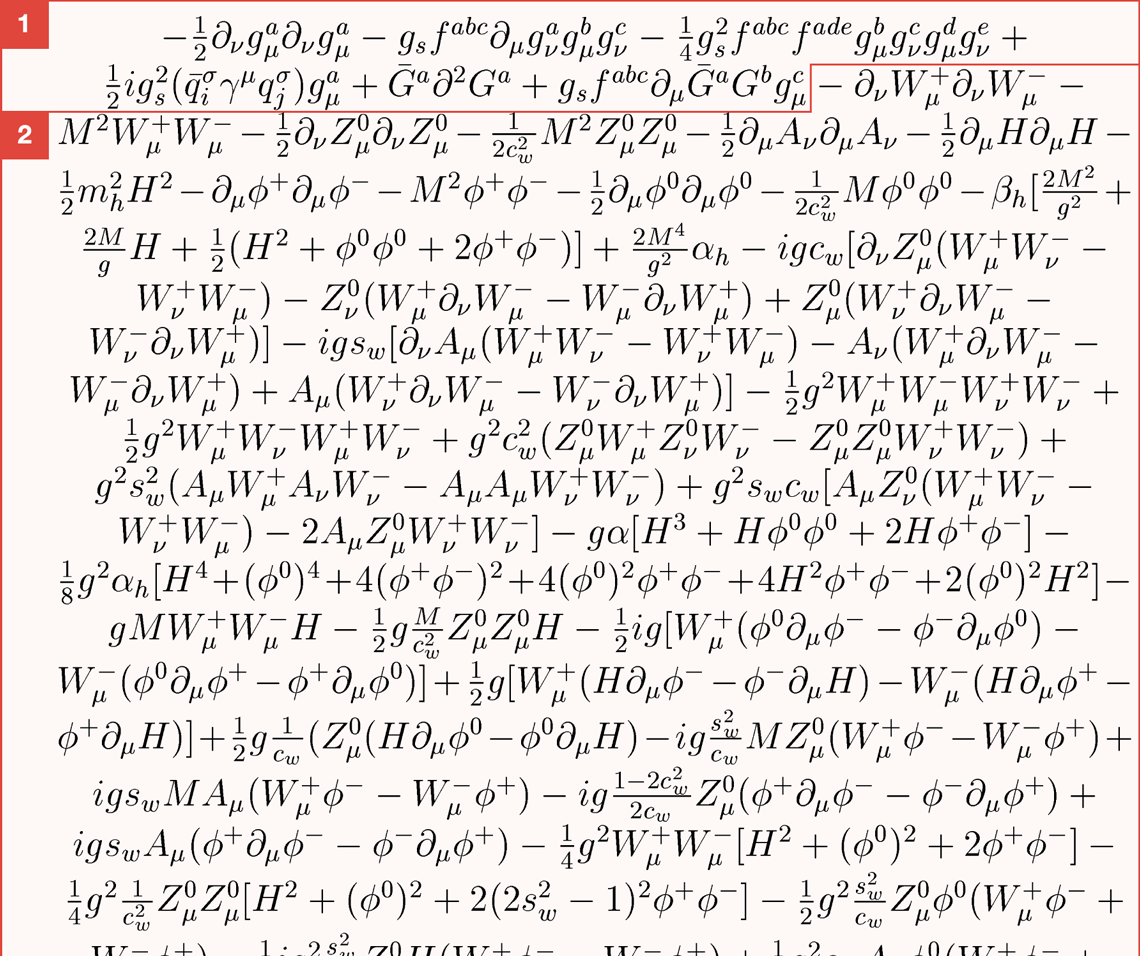
\includegraphics[width=0.49\linewidth]{/SM/image_part_001.png}
		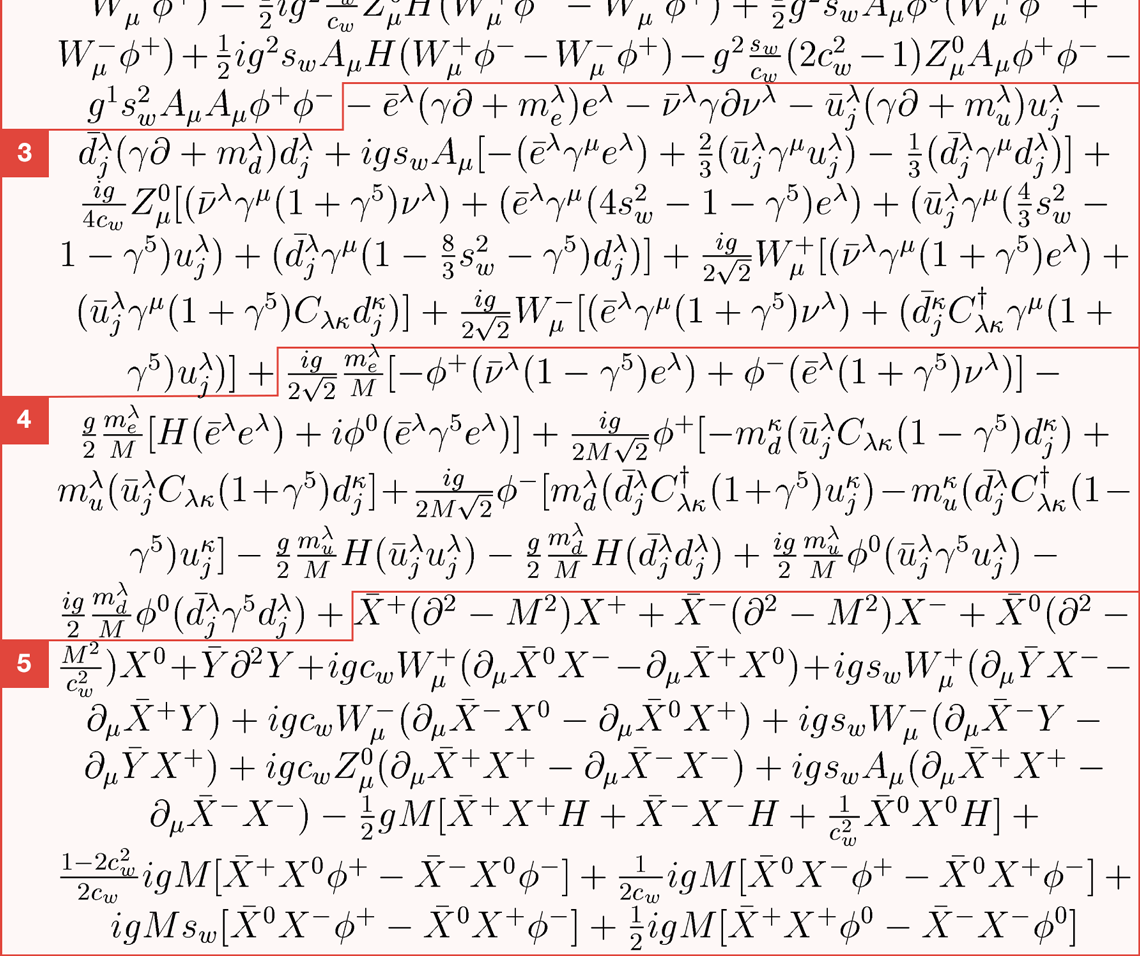
\includegraphics[width=0.49\linewidth]{/SM/image_part_002.png}
	\end{figure}

\end{frame}

\begin{frame}
	\frametitle{The Standard Model Lagrangian}
	\begin{figure}
		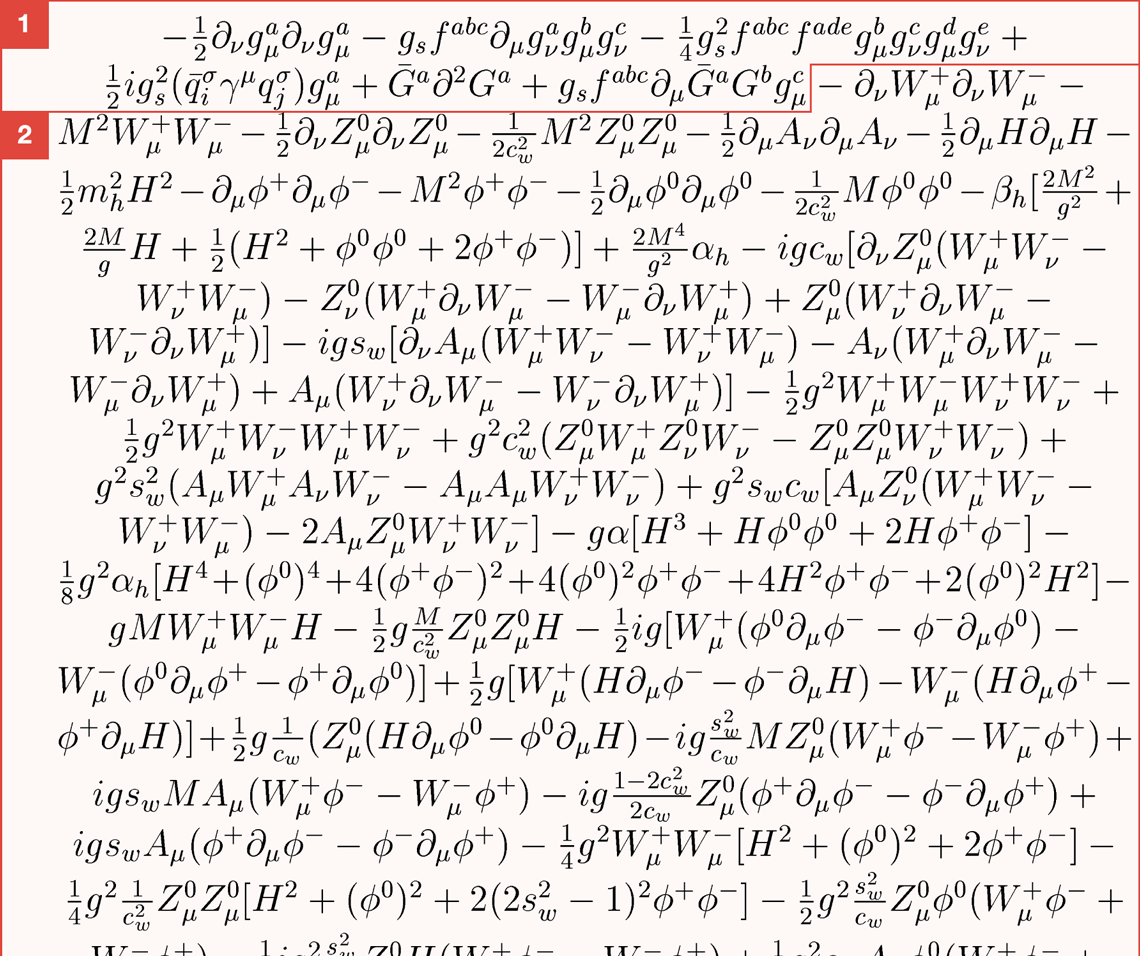
\includegraphics[width=0.49\linewidth]{/SM/image_part_001.png}
		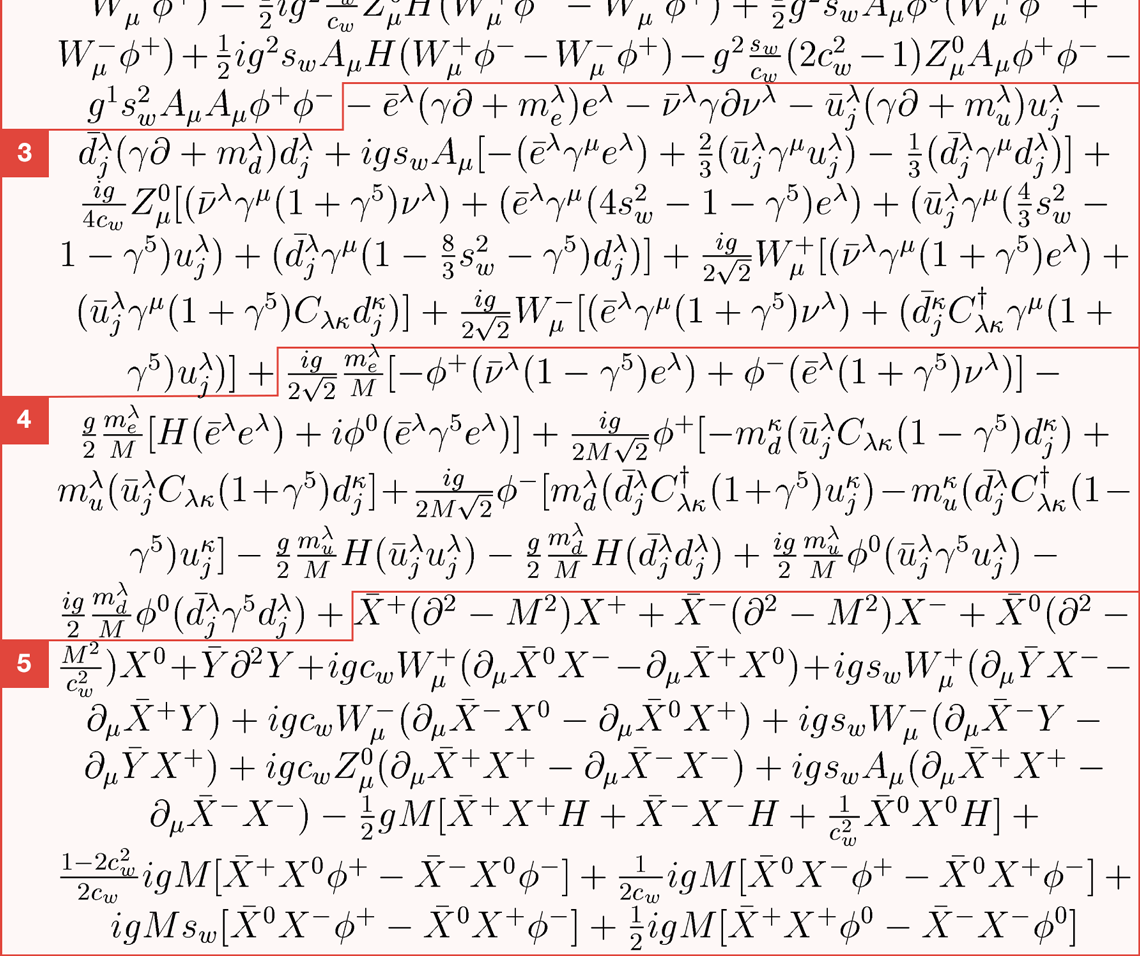
\includegraphics[width=0.49\linewidth]{/SM/image_part_002.png}
	\end{figure}

\begin{multicols}{2}
	\begin{enumerate}
		\item Gluon terms (Strong Force)
		\item W and Z terms (Weak force ) 
		\item Matter interactions with the weak force
		\item Ghosts (related to particle propagation)  
		\item Faddeev-Popov ghosts (gauge cancellations) 
	\end{enumerate}
\end{multicols}

\end{frame}

\begin{frame}
	\begin{itemize}
		\item Of course this is usually shortened to it's neat, mug compatible, form,
	\end{itemize}
	\begin{figure}
		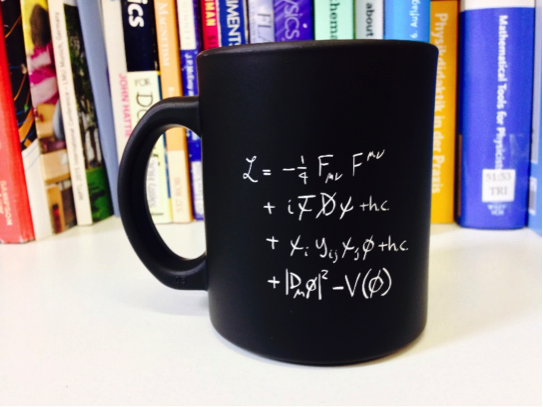
\includegraphics[width=0.65\linewidth,keepaspectratio]{SM/SM_Lagrangian_Mug.png}
	\end{figure}
	\begin{itemize}
	\item We do something similar and look at the SM in parts before looking at exactly these expressions represent.
\end{itemize}
\end{frame}

\begin{frame}
\frametitle{Higgs Mechanism}

\frametitle{Fields/Structure/HiggsVEV}
%
The SM is invariant under, 
%
\begin{equation}
\mathcal{G}_{SM} = \mathrm{SU}(3)_{\mathrm{C}} \times \mathrm{SU}_{\text{L}} \times \mathrm{U}_{\text{Y}}   .
\label{eq:SM_Group}
\end{equation} 
%
something
\begin{columns}
	\begin{column}{.55\textwidth}%
		\begin{equation}
		H = \begin{pmatrix}
		\phi_1 + i \phi_2 \\ 
		v + h + i \phi_3 
		\end{pmatrix}   \rightarrow  \langle H  \rangle =  \frac{1}{\sqrt{2}} \begin{pmatrix}
		0 \\ 
		v + h 
		\end{pmatrix}  .
		\label{shame}
		\nonumber
		\end{equation}
	\end{column}%
	\begin{column}{.45\textwidth}%
		\begin{figure}
			\centering
			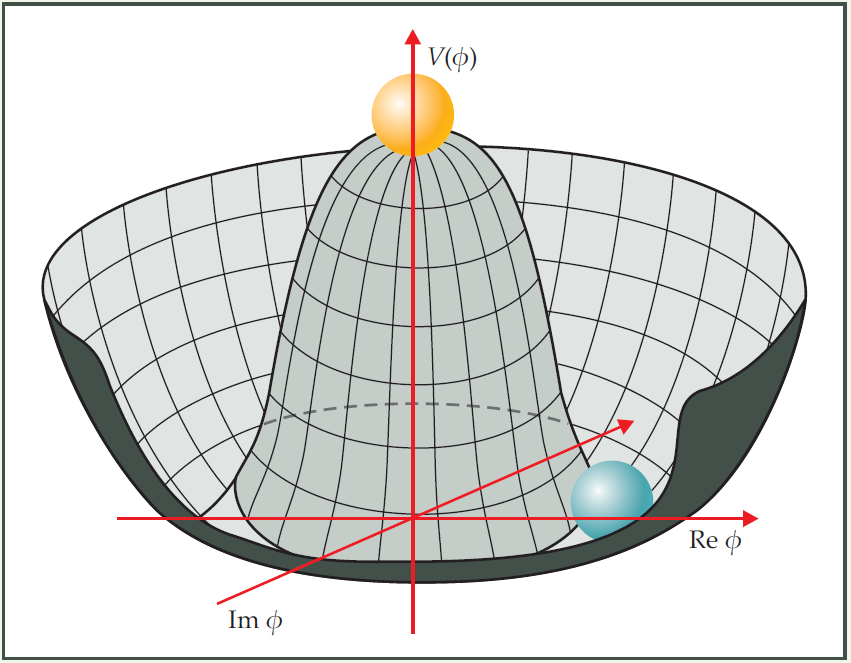
\includegraphics[width=0.9\textwidth,keepaspectratio]{SM/HiggsPot.png}
			\caption{Higgs Mechanism}
		\end{figure}
	
	\end{column}%
\end{columns}

\end{frame}

\begin{frame}
\frametitle{Gauge Terms and Bosons}

The portion of the Lagrangian that is of most import to the gauge bosons is, 
%
\begin{align}
\label{eq:KinSM}
\mathcal{L}_{kin} = & - \frac{1}{4} G^{\mu \nu}_a G_{a \, \mu \nu}  - \frac{1}{4}  A^{\mu \nu}_a A_{a \,\mu \nu}  
- \frac{1}{4}  B^{\mu \nu} B_{\mu \nu} \nonumber \\ 
& -i \bar{Q}_{L_i} \slashed{D} Q_{L_i} 
-i \bar{u}_{R_i} \slashed{D} u_{R_i}  
-i \bar{d}_{R_i} \slashed{D} d_{R_i}  
-i \bar{L}_{L_i} \slashed{D} L_{L_i}    
-i \bar{e}_{R_i} \slashed{D} e_{R_i}   \\
& - (D_\mu H)^\dagger ( D^\mu H ) ,  \nonumber 
\end{align}
This is before the Higgs mechanism gets in full effect. Being that the generation of mass comes from the interactions with the Higgs, we find the following terms, 
\begin{equation}
m_V^2 =
\dfrac{v^2}{4}
\begin{pmatrix}
g^2 \;\;&\;\; 0 \;\;&\;\; 0 \;\;&\;\; 0 \;\; \\
0 \;\;&\;\; g^2 \;\;&\;\; 0 \;\;&\;\; 0 \;\; \\
0 \;\;&\;\; 0 \;\;&\;\; g^2 \;\;&\;\; -g g_{Y} \;\; \\
0 \;\;&\;\; 0 \;\;&\;\; -g g_{Y} \;\;&\;\; g_{Y}^2 \;\; \\
\end{pmatrix} , 
\end{equation}
so we move to a eigenbasis, 
\begin{equation}
\begin{pmatrix}
	A_\mu^1 & A_\mu^2 & A_\mu^3 &  B_\mu
\end{pmatrix} \rightarrow \begin{pmatrix}

\end{pmatrix}
\end{equation}


\begin{equation}
\begin{pmatrix}
A_\mu^3 && B_\mu
\end{pmatrix} \cdot  \frac{1}{2} v^2 \begin{pmatrix}
g^2  & -g g^\prime \\
-g g^\prime & g^{\prime 2} 
\end{pmatrix} \cdot \begin{pmatrix}
A^{\mu,3} \\  B^\mu
\end{pmatrix}  , 
\end{equation} 
%
\begin{equation}
\begin{pmatrix}
A_\mu && Z_\mu 
\end{pmatrix} \begin{pmatrix}
0  & 0 \\
0  & \frac{1}{2} v \sqrt{g^2 + g^{\prime 2}} 
\end{pmatrix}  \begin{pmatrix}
A^\mu \\ Z^\mu
\end{pmatrix} , 
\end{equation}

\end{frame}

\begin{frame}

\end{frame}
	
	\begin{frame}
		\frametitle{Gauge Masses}
		content...
	\end{frame}
	
	\begin{frame}
		\frametitle{Flavor violation}
		content...
	\end{frame}
	
	\section{B-L-SM section} 
	
	\begin{frame}
	
	\frametitle{Differences given the fields}
	
	\textbf{Motivations for $\bm{\mathrm{B-L}}$ (Baryon number minus Lepton number) symmetry:}
	\vskip5mm
	\begin{itemize}
		\item The SM contains an accidental symmetry that conserves $\mathrm{B-L}$,
		\vskip2mm
		\item $\mathrm{B-L}$ symmetry relevant for baryogenesis through leptogenesis,
		\begin{itemize}
			\item sphaleron process violates $\mathrm{B}$ but preserves $\mathrm{B-L}$
		\end{itemize}  
		\item Grand Unified Theories, e.g.~$\SO{10}{}$, $\E{6}$, $\E{8},\ldots$ contain gauged $\U{B-L}$,
		\item The scale of $\U{B-L}$ breaking sets the mass scale of the right-handed Majorana neutrinos.
	\end{itemize}
	
	\end{frame}
	
\begin{frame}{BSM physics}
	
	\begin{itemize}
		\item \textbf{Three} generations of right-handed neutrinos $\to$ \textbf{\red no gauge anomalies}
		\begin{itemize}
			\item[>] Lightest is sterile and can be keV to TeV dark matter candidate. \\ {\blue \scriptsize  Kaneta, Kang, Lee: JHEP 1702 (2017) 031}
			\item[>] Or stabilized via a $\mathbb{Z}_2^{\mathrm{DM}}$
			\begin{itemize}
				\item[-] Annihilation via $Z^\prime$ portal {\scriptsize \blue Okada: Adv.High Energy Phys. 2018 (2018) 5340935}
				\item[-] Annihilation via Higgs portal {\scriptsize  \blue Okada, Seto: Phys.Rev. D82 (2010) 023507}
			\end{itemize}
		\end{itemize}
		\vskip2mm
		\item Model contains a complex-singlet scalar $\chi$ whose VEV breaks $\U{B-L}$
		\begin{itemize}
			\item[>] Scalar sector studies: {\scriptsize  \blue Basso, Moretti, Pruna: Eur.Phys.J. C71 (2011) 1724, Phys.Rev. D82 (2010) 055018}
			\vskip2mm
			\item[>] Enhanced vacuum stability compared to the SM
			
		\end{itemize}	
		\vskip2mm
		\item Model contains an extra $Z^\prime$ gauge boson {\scriptsize  \blue Basso, Belyaev, Moretti, Pruna: JHEP 0910 (2009) 006} ; {\scriptsize  \blue Basso, Belyaev, Moretti, Shepherd-Themistocleous: Phys.Rev. D80 (2009) 055030}
		%			\begin{itemize}
		%				\item[>] \textbf{BSM vector bosons contribute to $\bm{\(g-2\)_\mu}$ anomaly}
		%				%%%%%%%%%%%%%%%%%%%%%%%%%
		%				\begin{figure}[!h]
		%					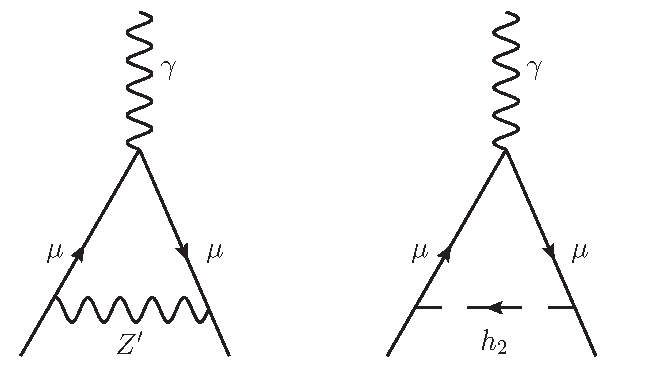
\includegraphics[scale=0.4]{g-2.pdf}
		%				\end{figure}	
		%				%%%%%%%%%%%%%%%%%%%%%%%%%
		%				\item[>] {\bf \red Not studied in the B-L SM} (recently addressed in the B-L SSM \\ {\scriptsize \blue Yang, Feng et al. Phys.Rev. D99 (2019) no.1, 015002})
		%			\end{itemize}
		
	\end{itemize}
	
	
	\end{frame}

	\begin{frame}
		\frametitle{R1}
		\begin{equation*}
			\begin{aligned}
			\begin{pmatrix}
			h_1 \\
			h_2 
			\end{pmatrix}
			=
			\begin{pmatrix}
			\cos \alpha_h & -\sin \alpha_h \\
			\sin \alpha_h & \cos \alpha_h 
			\end{pmatrix}
			\begin{pmatrix}
			h \\
			h^\prime 
			\end{pmatrix}
			\end{aligned}
		\end{equation*}
		\vskip0.1mm
		{\bf Heavy $Z^\prime$ implies that $\bm{x \gg v}$ for most of the parameters points:}
		\begin{equation*}
			\sin \alpha_h \approx \dfrac{1}{2}\dfrac{\lambda_3}{\lambda_2} \dfrac{v}{x} \qquad
			m_{h_1}^2 \approx 2 \lambda_1 v^2 \qquad m_{h_2}^2 \approx 2 \lambda_2 x^2
		\end{equation*}
		\begin{exampleblock}{}
		Kinetic mixing
		\end{exampleblock}
		\begin{equation*}
		\begin{aligned}
		\mathcal{L}_\mathrm{bosons} =  \abs{D_\mu H}^2 + \abs{D_\mu \chi}^2 - V\(H,\chi\) -\dfrac{1}{4} F_{\mu \nu} F^{\mu \nu} -\dfrac{1}{4} F^\prime_{\mu \nu} F^{\prime \mu \nu} -\dfrac{1}{2} \kappa F_{\mu \nu} F^{\prime \mu \nu}
		\end{aligned}
		\end{equation*}
		
		\begin{itemize}
			\item $\kappa$ is a ${\green \U{Y}} \times {\red \U{B-L}}$ gauge
			kinetic-mixing parameter
			\vskip2mm
			\item Field strength tensors ${\green F_{\mu \nu} = \partial_\mu A_\nu - \partial_\nu A_\mu}$ and ${\red F^\prime_{\mu \nu} = \partial_\mu A^\prime_\nu - \partial_\nu A^\prime_\mu}$
			\item {\blue Redefine $\kappa = \sin \alpha$ and gauge fields as (convenient basis choice)}
			\begin{equation*}
				\begin{pmatrix}
				A_\mu \\
				A^\prime_\mu 
				\end{pmatrix}
				=
				\begin{pmatrix}
				1 & -\tan \alpha \\
				0 & \sec \alpha 
				\end{pmatrix}
				\begin{pmatrix}
				B_\mu \\
				B^\prime_\mu 
				\end{pmatrix}\,,
				\label{eq:trans-kappa}
			\end{equation*}	
			\item Kinetic terms acquire canonical form
			\begin{equation*}
				\begin{aligned}
				\mathcal{L}_\mathrm{kinetic} =   -\dfrac{1}{4} B_{\mu \nu} B^{\mu \nu} -\dfrac{1}{4} B^\prime_{\mu \nu} B^{\prime \mu \nu}
				\end{aligned}
				\end{equation*}					
		\end{itemize}
		
		
		\begin{exampleblock}{}
			{\bf Gauge kinetic-mixing induces mixing between $Z^\prime$, $Z$ and $\gamma$ }
		\end{exampleblock} 
		
		\begin{equation*}
			\begin{aligned}
			\begin{pmatrix}
			\gamma_\mu \\
			Z_\mu \\
			Z^\prime_\mu
			\end{pmatrix}
			=
			\begin{pmatrix}
			\cos \theta_W & \sin \theta_W & 0\\
			-\sin \theta_W \cos \theta_W^\prime & \cos \theta_W \cos \theta_W^\prime & \sin \theta_W^\prime \\
			\sin \theta_W \sin \theta_W^\prime & -\cos \theta_W^\prime \sin \theta_W^\prime & \cos \theta_W^\prime
			\end{pmatrix}
			\begin{pmatrix}
			B_\mu \\
			A^3_\mu \\
			B^\prime_\mu
			\end{pmatrix}
			\end{aligned}
		\end{equation*}
	
	\end{frame}
	

\begin{frame}{Yukawa sector}
	\begin{equation*}
	\begin{aligned}
	\mathcal{L}_\mathrm{Yukawa} = 
	-y_u^{ij} \overline{q_\mathrm{L i}} u_\mathrm{R j} \widetilde{H} 
	-y_d^{ij} \overline{q_\mathrm{L i}} d_\mathrm{R j} H
	-y_e^{ij} \overline{\ell_\mathrm{L i}} e_\mathrm{R j} H
	{\red - y_\nu^{ij} \overline{\ell_\mathrm{L i}} \nu_\mathrm{R j} \widetilde{H}
		-\dfrac{1}{2} y_M^{ij} \overline{\nu_\mathrm{R i}^c} \nu_\mathrm{R j} \chi} + \mathrm{c.c.}
	\end{aligned}
	\end{equation*}
	\begin{itemize}
		\item $\widetilde{H} = i \sigma^2 H^*$
		\vskip2mm
		\item Dirac and Majorana masses matrices: $\bm{m_D} = \tfrac{\bm{y_\nu}}{\sqrt{2}} v$ and $\bm{M} = \tfrac{\bm{y_M}}{\sqrt{2}} x$
		\item Neutrino masses via see-saw mechanism: $\begin{pmatrix}
		0 & m_D \\
		m_D & M\\
		\end{pmatrix} \rightarrow 
		\begin{cases}
		m_{\nu_l} \approx \tfrac{m_D^2}{M}\\
		m_{\nu_h} \approx M
		\end{cases}$
		\item Small mixing angle: $\tan \alpha_\nu \approx -2 \sqrt{\tfrac{m_{\nu_l}}{m_{\nu_h}}}$
	\end{itemize}
	
\end{frame}

	
	\begin{frame}
		\frametitle{R3}
		content...
	\end{frame}
	
	\section{3HDM section}
	
	\section{Extra information}
	
	\section{Help and learning}

	%\begin{frame}
		%\frametitle{Help: Column}
		
		%\begin{columns}
		%	\column{.5\textwidth}
		%	text 
		%	\column{.5\textwidth}
		%	side text~
		%\end{columns}
	%\end{frame}
	
	%\begin{frame}
		%\frametitle{Itemize}
		
		%\begin{itemize}
			%\item A 
			%\item B 
			%\begin{enumerate}
			%	\item B-1 
			%	\item B-2 
			%\end{enumerate}
		%\item C	
	%\end{itemize}
		
	%\end{frame}
	
\end{document}